
\documentclass[sigconf, nonacm=true]{acmart}
\setcopyright{none}
%\documentclass[9pt,twocolumn]{extarticle}
%\usepackage[a4paper,margin=0.8in]{geometry}
%\usepackage{dblfloatfix}
%\usepackage{graphicx}
\usepackage{tabularx}
%\usepackage[T1]{fontenc}
%\usepackage{tgschola}

\begin{document}
\title{ECOLM Futures Review}

\author{Chris Cannam}
\orcid{https://orcid.org/0009-0001-9814-6512}
\affiliation{%
  \institution{Particular Programs Ltd}
  \city{London}
  \country{UK}}
\email{chris.cannam@particularprograms.co.uk}

\author{David Lewis}
\affiliation{%
  \institution{Goldsmiths, University of London}
  \city{London}
  \country{UK}}
\email{d.lewis@gold.ac.uk}

\author{Tim Crawford}
\affiliation{%
  \institution{Goldsmiths, University of London}
  \city{London}
  \country{UK}}
\email{t.crawford@gold.ac.uk}

\maketitle
\begin{sloppypar}
  
  %\begin{abstract}
  %\end{abstract}

  \begin{itemize}
    \item {\bf STATUS Preliminary thought-dump}
    \item {\bf TODO Eliminate almost all of the bulleted lists, turning into
      prose or something else such as tables}
  \end{itemize}
  
  \section{Background and Motivation}

  \subsection{What is ECOLM?}

  ECOLM\footnote{http://igor.gold.ac.uk/isms/ecolm/} or ``Electronic
  Corpus of Lute Music'' was a series of research projects aiming to
  develop a queryable online database of lute tablature encodings, of
  quality suitable for scholarly use.

  Two critical, and still relevant, goals were:
  
  \begin{enumerate}
  \item To store and deliver encodings of music, not only metadata;
  \item To be trustworthy for scholarly use: for example, sources are
    identified, reliability of attribution is noted, editorial changes
    are pointed out, and the schema distinguishes between performance
    and diplomatic transcriptions.
  \end{enumerate}
  
  Here we use the name ECOLM broadly to refer to this design of
  database application, as well as to the past research projects of
  that name and to the existing
  system\footnote{http://doc.gold.ac.uk/isms/ecolm/database/} that
  they produced.

  \subsection{Aim and Structure of this Review}

  We aim to review the premise and outcomes of ECOLM and to consider
  whether a ``lightweight path to sustainability'' can be found that
  can be incrementally extended to other tablature resources.

  In section \ref{enumerate-resources} we first set out the history of
  ECOLM and enumerate other resources of interest. Section
  \ref{user-context} identifies some typical users of such resources
  and describes our findings from user interviews. In section
  \ref{technical} we outline the technical makeup of each of these
  resources and some related sites of interest. Section
  \ref{desirable-qualities} summarises the desirable qualities we seek
  in a solution, and section \ref{future} suggests three possible
  future courses of action.

  \section{ECOLM and Other Resources}\label{enumerate-resources}
  
  \subsection{The ECOLM Projects}

  %%%!!! + bibliography
  %%%!!! + URLs in footnote
  \begin{itemize}
  \item {\bf ECOLM} (1999-2002) was a project run by Tim Crawford,
    initially at King's College London, which produced a queryable
    database of lute encodings with metadata with a web interface. The
    resulting service is still accessible today through a
    public-facing server hosted at Goldsmiths.
  \item {\bf ECOLM II} (2002-2006) was a successor project which
    expanded the ECOLM database and used it for some computational
    musicological investigations.
  \item {\bf ECOLM III} (2012) was a short project with the goal of
    adding further high-quality encodings by crowd-sourcing
    corrections of OMR (optical music recognition) scans.
    %%%!!! say more about this later
  \end{itemize}

  The ECOLM database as available online contains about 2,000
  tablature encodings, manually curated, of relatively high quality
  with accompanying metadata.

  \subsection{Other Lute Tablature Resources}

  Several other collections of lute music have been collected and
  placed online by various curators. Of particular interest are:
  \begin{itemize}
    \item {\bf Mss.slweiss.de}\footnote{https://mss.slweiss.de/}
      curated by Peter Steur and the late Markus Lutz. A metadata
      catalogue of around 68,000 listings of which the majority have
      incipits (opening ideas) encoded.
    \item {\bf Lutemusic.org}\footnote{https://lutemusic.org/} curated
      by Sarge Gerbode. Around 20,000 encodings in playing editions
      with semi-structured metadata, informally curated with limited
      version tracking or editorial notes.
    \item {\bf Lute Society publications} curated by John
      Robinson. Scans from printed periodicals intended for players,
      containing around 7,000 encodings consisting of printed music,
      prose commentary, and semi-structured metadata.
    \item {\bf Phal\`ese} curated by Jan Burgers. Around 1,000
      encodings transcribed from editions of 16th-century publisher
      Pierre Phal\`ese with publication metadata.

      %%!!! tabulate their type, content, whether published already,
      %% licence terms, how widely used
  \end{itemize}

  There are concerns about the ongoing sustainability of all of these,
  similar to those about ECOLM: curation and maintenance by
  individuals or small groups of enthusiasts, in some cases of
  retirement age; maintenance in limited periods of spare time,
  perhaps following initial short-term funding; data management using
  ad-hoc methods or private systems that are not accessible to
  third-party reproduction; lack of data export facilities or support
  for common interchange formats.

  Therefore, we would prefer to find a solution with the potential to
  incorporate and maintain data from these resources as well.

  The lutemusic.org transcriptions are explicitly Creative Commons
  NC-SA licensed, and the maintainers of the other listed resources
  have indicated willingness to contribute to a potential combined
  dataset.
  
  \renewcommand{\arraystretch}{1.2}
  \setlength{\tabcolsep}{4pt}
  
  \begin{table*}[t]
  \caption{Status of data and metadata in online lute tablature resources}
  \small
      \begin{tabularx}{\textwidth}{|l|X|X|X|X|X|X|X|X|X|}
        \hline
        & \multicolumn{4}{|c|}{\bf Data} & \multicolumn{5}{|c|}{\bf Metadata} \\
        \hline
        & Encoded tablature & OTR scanned pages & Facsimile images & Published PDFs
        & Works linked to encodings & Ordered work-lists & Textual commentary & Textual references to models & Structured metadata \\
        \hline
            {ECOLM I/II} & Yes & Partial & Yes & & Yes & Yes & & Partial & Yes \\
        \hline
            {Mss.slweiss.de} & Yes & & & & & Yes & & & Partial \\
        \hline
            {Lutemusic.org} & Yes & & Partial & Yes & Partial & & & & Partial \\
        \hline
            {Lute Society} & Yes &  & & Yes & & Yes & Yes & Yes & \\
        \hline
            {Phal\`ese} & Yes & & & Yes & Partial & Partial & Yes & Yes & \\
            \hline
      \end{tabularx}
  \label{table:datasets}
  \end{table*}
  
  %%!!! include section about other non-lute resources: RISM being the
  %%!!! most obvious but also anything else anyone else mentioned
  
  \section{Understanding User Context}\label{user-context}

  We conducted informal interviews with three exemplary users of
  online early-music resources, in order to understand scholarly
  expectations. These were a ``traditional'' musicologist, a
  computational musicologist, and a lute performer and teacher.
  
  \subsection{Musicologist}

  The musicologist gave the following indications about their use of
  online resources of this type:

  \begin{itemize}
    \item Depending on the material, may begin by searching
      RISM\footnote{https://rism.info/} or
      Cantus\footnote{https://cantus.uwaterloo.ca/} databases;
    \item Routinely starts with a search by composer or source, since
      titles tend to have too many historical variants;
    \item Finds diplomatic transcriptions (i.e. closely following
      the source without editorial intervention) the most useful,
      but grateful for any transcription;
    \item Always refers to the facsimile as well, regardless of status
      of transcriptions, so can often do without editorial notes;
    \item Is particularly interested in dual tablature and staff
      renderings;
    \item Would appreciate opportunity to annotate or correct
      unreliable transcriptions.
  \end{itemize}
  
  \subsection{Computational Musicologist}

  The computational musicologist gave the following indications about
  their use of such resources:

  \begin{itemize}
  \item Will typically begin by searching RISM, and trusts that
    metadata in RISM is more authoritative than elsewhere;
  \item Finds trust very important, appreciating annotations about the
    original source, transcriber, and editorial interventions;
  \item Can work with unreliable transcriptions if their quality is
    known and original sources are properly described;
  \item Appreciates a simple presentation and single search function
    as their first entry point;
  \item Finds the ability to refine results via facets more useful
    than the ability to construct complex queries from the outset;
  \item Wants the ability to download results (up to the whole
    dataset) or query via API, to use with computational tools such
    as music21 or Humdrum locally.
  \end{itemize}
  
  \subsection{Lute Performer and Teacher}

  The lute performer and teacher gave the following indications about
  their use:

  \begin{itemize}
    \item Will often begin using the most informal performance
      resources because they have the most material, but this causes
      problems cross-referencing with more authoritative material;
    \item Finds information about the original source, transcriber,
      editorial interventions extremely important;
    \item Expects students to know those things about the editions
      they use when performing;
    \item Would greatly appreciate something containing modern
      performing editions as at lutemusic.org but with more reliable
      editorial commentary;
    \item In the absence of trustworthy information about the
      transcription, needs to compare every note with facsimile before
      using.
  \end{itemize}

  \subsection{Common Threads}

  Trust and provenance are common themes in discussion with all three
  of our exemplary users. They have different requirements for
  content, format, detail of editorial notes and so on, but share a
  desire to know the quality of transcription and level of editorial
  intervention they are dealing with.

  There was also some consensus about the value of simple search with
  subsequent refinement, of a cleanly-designed results layout
  including inline incipits, and of API and data provision.
  
  The musicological specialists were comfortable with RISM and would
  prefer some level of compatibility, perhaps as far as having the
  works indexed from RISM and metadata managed there.

  None of the three indicated they would hope to {\em contribute}
  material to a dataset like this, although they might appreciate the
  ability to make corrections.
  
  \section{Technical Review}\label{technical}

  \subsection{Tablature Resources}
  
  \subsubsection{ECOLM}

  \begin{itemize}
  \item SQL database
  \item Entity relationships modelled in schema---pre-RDF, not
    triples, relations hardcoded
  \item Structured using ``clusters'' (give examples)---attempt to
    support more general relations within schema
  \item Confidence levels modelled
  \item Same database used for user logins / editorial control as for
    content records---expectation that data managed ``within ECOLM''
  \item Degree of rigour in organisation means that, while it may be
    tricky to convert or adapt to another format or system, such an
    effort will probably succeed without too many loose ends
  \end{itemize}

  See section \ref{ecolm-data} for more technical details.

  \subsubsection{mss.slweiss.de}

  \begin{itemize}
  \item PHP web application driven entirely from CSV files (actually
    semicolon-separated rather than comma-separated)
  \item Flat directory containing one CSV file per source
  \item Incipits embedded in the CSV files, in ABC format, rendered to
    SVG from the PHP scripts for serving to browser
  \item Separate index CSV files list manuscript metadata and
    concordances
  \item Version-controlled since 2013
  \item Organisation seems tidy and easy to deal with
  \end{itemize}
  
  \subsubsection{lutemusic.org}

  \begin{itemize}
  \item Hierarchical organisation with separate trees by composer,
    source, and facsimile
  \item Composer and source trees contain Fronimo tab transcriptions
    with derived MIDI and PDF renderings
  \item Facsimile tree contains images (typically PNG) closely cropped
    with thresholding, apparently intended for reading from screen
    rather than as historical page facsimiles
  \item Separate tab hierarchy also present with tab-format files,
    probably older
  \item Hand-maintained spreadsheet contains metadata and index for
    Fronimo files
  \item Website presents the filesystem hierarchy directly (entirely
    static, uses web server index pages, nothing generated)
  \item Irregular organisation may make adaptation relatively high
    risk
  \end{itemize}
    
  \subsubsection{Lute Society}

  \begin{itemize}
  \item Lute News facsimiles and transcriptions organised by issue
  \item Organisation is on filesystem, with PDFs and transcriptions of
    both text and tablature
  \item Simple front-end added by Tim
    Crawford\footnote{https://doc.gold.ac.uk/~mas01tc/jhr\_web/}
    provides a web index via Javascript requests from client
  \item Seems well arranged, the biggest problem looks like the wide
    variety of types of material present and the original linear
    organisation for readers and players
  \end{itemize}
  
  \subsubsection{Phal\`ese}

  \subsection{Other Sites of Interest}
  
  \subsubsection{RISM}

  RISM\footnote{https://rism.info/} (R\'epertoire International des
  Sources Musicales) is a catalogue of musical sources. It ``documents
  what exists and where it is
  kept''\footnote{https://opac.rism.info/main-menu-/kachelmenu/about}. That
  is, it is not a library but an index of libraries and the sources
  they contain. It has a historical focus on physical sources rather
  than abstract works (although this may be changing) and although
  some records have incipits attached, it does not otherwise serve
  musical content.

  As we saw in section \ref{user-context}, musicologists routinely
  expect sources to be indexed in RISM and may expect it to offer the
  most authoritative source metadata.

  The RISM project also publishes a web application for entry and
  management of musical source catalogue data, called Muscat. See
  section \ref{muscat-data} for details about the schema used by
  Muscat.

  RISM records are stored in MARC\footnote{https://www.loc.gov/marc/}
  (Machine Readable Cataloging) format and are available as MARC or
  RDF data via API.

  \subsubsection{DIAMM}

  DIAMM\footnote{https://www.diamm.ac.uk/} (Digital Image Archive of
  Medieval Music) is an archive of scanned manuscripts, mainly from
  before 1600. It also indexes sources whose images are stored
  elsewhere. Images are typically of high quality with accompanying
  metadata describing the physical artifact in some detail.

  DIAMM has an API providing metadata in a JSON encoding, though
  apparently not RDF or JSON-LD.
  
  \subsubsection{Vihuela Database}

  The Vihuela Database\footnote{https://vihuelagriffiths.com/} of John
  Griffiths is a research-focused index of vihuela music and
  information about the vihuela. It includes a browseable and
  searchable list of pieces with incipits in image form and some text
  commentary. Significant fantasia themes are indexed separately by
  melody. The site does not appear to offer an API or data linking.

  Our consulted lute performer/teacher praised this site for its clear
  presentation of search results with inline incipits (figure
  \ref{fig:vihuela}) and use of editorial commentary.
  
  \begin{figure}[h]
  \centering
  \caption{Vihuela Database search results example}
  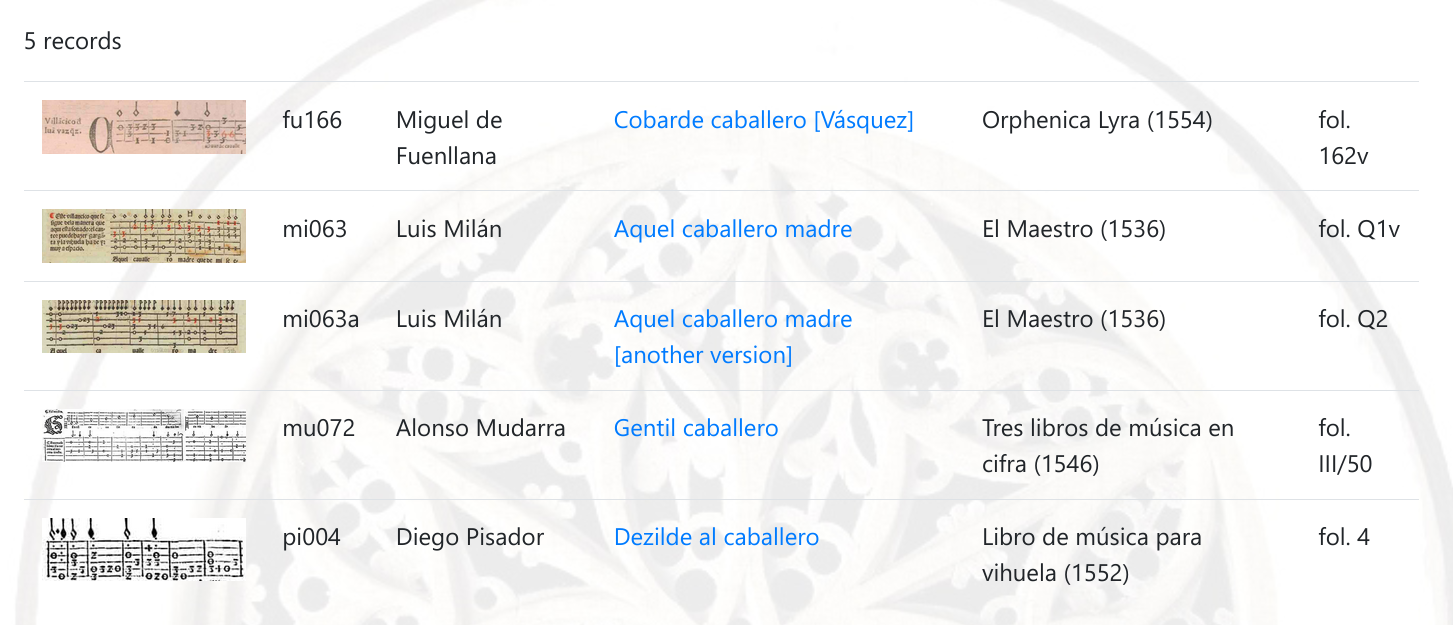
\includegraphics[width=\columnwidth]{images/vihuela-search-results}
  \label{fig:vihuela}
  \end{figure}
  
  \subsubsection{Josquin Research Project}

  The Josquin Research Project\footnote{https://josquin.stanford.edu/}
  from Jesse Rodin and Craig Sapp at Stanford is an index of early
  polyphonic music with full digitised scores. It is driven from a
  transparent catalogue of Humdrum-format scores, maintained under
  version control in a Git repository with a submodule per composer
  and available from the website in-page or via an API.

  Our consulted computational musicologist praised this site for its
  straightforward search interface, presentation of results including
  useful details such as vocal range plots, and publication of raw
  data for computational use.
  
%  \subsubsection{earlymusicsources.com}
%  \subsubsection{earlymusiconline.org}
  \subsubsection{IMSLP / Petrucci}

  IMSLP (the International Music Score Library Project or Petrucci
  Music Library) is a very widely used crowd-sourced library of
  public-domain and Creative Commons licensed sheet music. Managed
  using MediaWiki, it makes a priority of encouraging community
  contributions over authoritative editorial review. Works are often
  available in multiple versions including scans and transcriptions,
  typically rendered as PDFs rather than in machine-readable
  form. Depending on the composition, works may feature in full score,
  parts, and arrangements, and tablature often appears where
  applicable. There is some linkage to other informal resources such
  as Wikipedia as well as to formal authorities such as VIAF.
  
  \section{Desirable Qualities of a Solution}\label{desirable-qualities}
  \subsection{Social}

  \begin{itemize}
  \item talk about types of user and their expectations
  \item talk about crowdsourcing and ECOLM III
  \end{itemize}

  
  \subsection{Technical}

  \subsubsection{Required}
  
  \begin{itemize}
  \item ability to continue to absorb upstream changes, for
    adaptations of datasets that are also being maintained elsewhere
  \item standard formats where they exist! e.g. always MEI unless
    there's some very good reason
  \item automated testing for format conversions (e.g. from external sources)
  \item data served through API
  \item stable identifiers for works {\em and} for transcriptions, so
    that the latter can be used in principle by other services
    e.g. similarity
  \item disambiguation of sources among multiple datasets
  \item clear relation to identifiers in other sources (online or
    offline) where available
    \begin{itemize}
    \item particularly, cross-reference to RISM identifiers for
      composers and sources (where they exist)
    \end{itemize}
  \item ability to handle substantial textual and other unstructured
    data including diagrams and multimedia

  \end{itemize}

  \subsubsection{Desired}
  
  \begin{itemize}
  \item RDF
  \item possibly ``immutable pipeline'' - rebuildable from source
    format that is friendly for humans to work with
    \begin{itemize}
      \item but note the formats that other maintainers actually choose to
        use! CSV (probably exported from a spreadsheet) and
        XLS... much as I like e.g. RDF/Turtle, few people want to edit
        that or JSON-LD directly
    \end{itemize}
  \item ability to provide more than one front-end
  \item multiple types of facsimile as well as potentially of
    transcription---for example if a source has both Gerbode-edited
    PNG and a detailed scan with limited editing, it would be useful
    to retain both, with suitable metadata
  \item RISM indexing compatibility
  \item natively version-controlled
  \end{itemize}

  
  \subsection{User Experience}

  \section{Possible Paths}\label{future}

  \subsection{``Enhanced ECOLM''}

  Relational database derived from current ECOLM

  Advantages

  \begin{itemize}
  \item preserves existing code; first set of data already imported
  \item somewhat structured, encouraging consistency
  \item some good domain-specific decisions made in the schema design
  \item importing other data is work in the mature field of ETL with
    corresponding tooling etc
  \item can focus on user interfaces and data conversion rather than
    rebuilding representation from scratch
  \end{itemize}

  Disadvantages

  \begin{itemize}
  \item versioning is difficult
  \item does not solve the stable identifiers problem
  \item has proven somewhat overspecified for its current use
    (e.g. data maturity fields bodged)
  \item little in common with other solutions people have used, so all
    import/export is custom
  \item cannot easily drop in other ``views'' apart from any we have
    written ourselves
  \item providing APIs is manual work
  \end{itemize}

  \subsection{Graph-based}

  Fundamental representation is a graph of triples in the RDF mould;
  all metadata converted to that for import and from it for query;
  data such as transcriptions, multimedia etc referred to by
  identifiers in the same space (e.g. URIs)

  Advantages

  \begin{itemize}
    \item widely understood model, not least because other systems
      often make RDF available via API. Although no longer trendy, RDF
      has not died out and probably won't do soon
    \item lowest-common-denominator representation as target for data
      conversions
    \item not too awful for versioning (even just using git, with
      Turtle or JSON-LD)
    \item good target for ``idempotent'' one-way conversion flows,
      supporting automated tests for reliability, offering possibility
      to integrate ongoing upstream changes
    \item makes serving data via API almost free
    \item in principle can use existing tools for review, query,
      inferencing, format conversion
  \end{itemize}

  Disadvantages

  \begin{itemize}
    \item in practice using existing tools for inferencing means
      entering the world of galaxy-brained semantic web savants
    \item normal people do not choose to hand-maintain data in triples
      of URIs, so none of our candidate datasets use this format ---
      it's no CSV
    \item commonplace ontology mismatch giving ``silently missing
      data'' problems on query --- good testing strongly advised
    \item similarly, typeless or with awkward typing
    \item problem of which ontology to target does not appear to have
      a single best solution (and we don't really want to be in the
      business of developing one)
    \item no built-in solution to problem of identifying and
      retrieving bulkier data such as images
  \end{itemize}

  \subsection{``RISM-aligned''}

  Fundamental metadata representation is MARC, and we use Muscat to
  maintain it? 
  
  \clearpage

  \section{Data representation in existing systems}
  
  \subsection{ECOLM II}\label{ecolm-data}
  
  \begin{figure*}[b]
  \centering
  \caption{ECOLM II database schema (record tables)}
  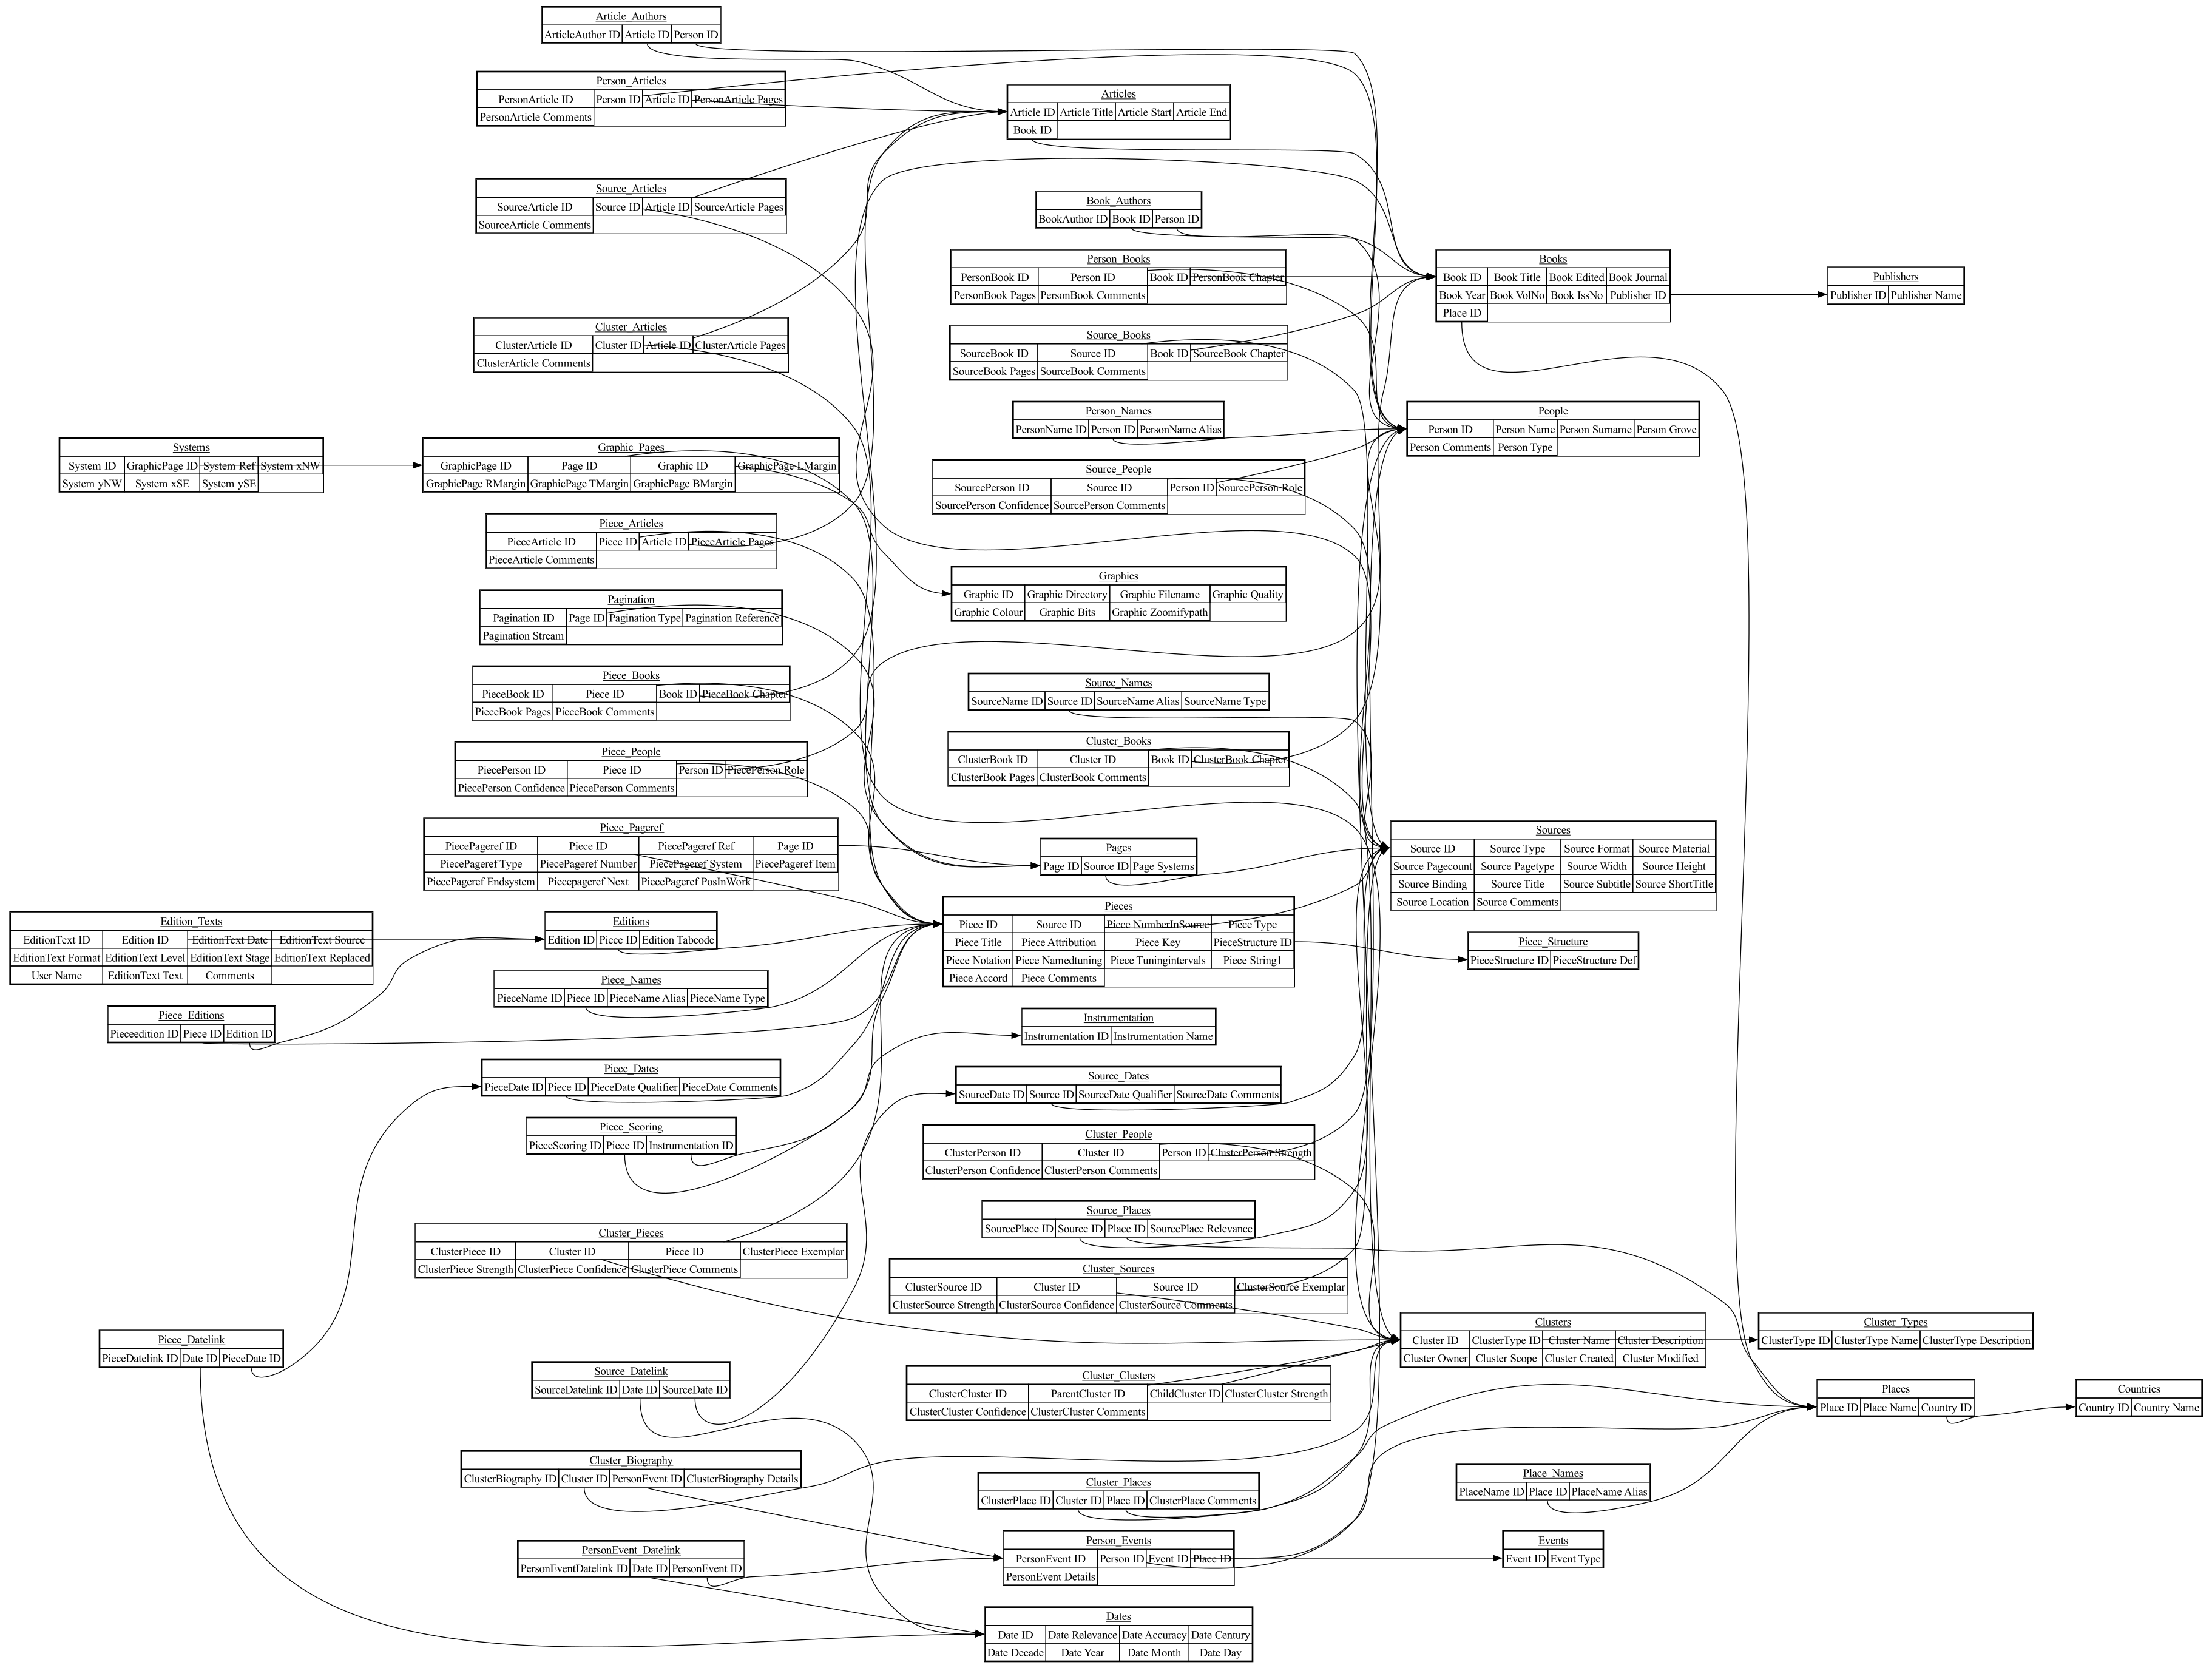
\includegraphics[width=\textwidth]{plot/records}
  \label{fig:records}
  \end{figure*}

  ECOLM I and II store all data directly in a relational database. The
  database contains both editorial tables, about users of ECOLM and
  their contributions, and record tables, about the works in the
  dataset. Figure \ref{fig:records} shows the record tables.

  The schema models join relationships using either foreign keys
  (e.g. {\tt Source ID} in {\tt Pieces}) or join tables (e.g. {\tt
    Person\_Events}) depending on the presence of metadata about the
  relationship.

  ECOLM has specific definitions of ``piece'' and ``work''. A piece is
  ``a single musical entity within a specified source'', while a work
  is ``a cluster of pieces in different sources that all represent the
  same musical work''. The database also uses ``cluster'' to record
  groups other than works. For example, the ECOLM II database contains
  only 9 ``pieces'' directly linked to John Dowland as composer or
  scribe, but 109 ``pieces'' linked to him through clusters: 105 as
  members of the Lachrimae ``group'' cluster, and 4 others through
  ``work'' clusters.

  The ECOLM schema is unusual today in using mixed-case naming with
  spaces in the column names.
  
  \clearpage

  \subsection{RISM Muscat web application}\label{muscat-data}
  
  \begin{figure*}[b]
  \centering
  \caption{RISM Muscat schema summary}
  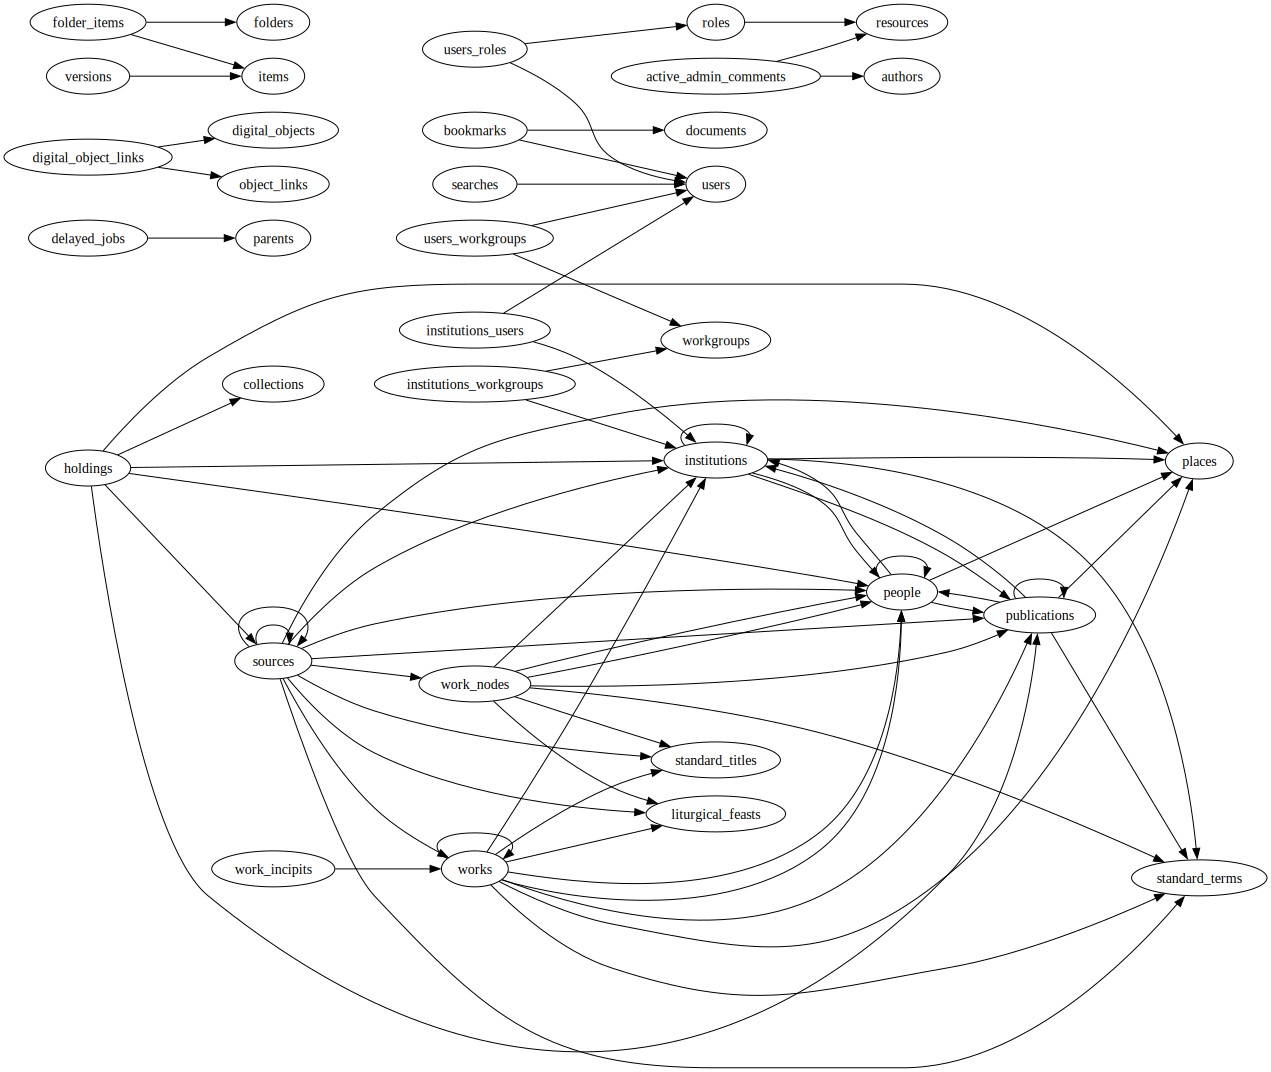
\includegraphics[width=\textwidth]{plot/muscat}
  \label{fig:muscat}
  \end{figure*}

  Muscat\footnote{https://rism.info/community/muscat.html} is a web
  application published by RISM for cataloguing musical sources,
  written using Ruby on Rails. Figure \ref{fig:muscat} shows the main
  tables.

  Muscat uses a hybrid schema, in that each table has a single {\tt
    marc\_source} column containing an authoritative record in
  MARC21\footnote{https://www.loc.gov/marc/} concise text format. Most
  of the other columns are apparently used to ``cache'' data from the
  MARC record that may be needed quickly for display or search. At
  core, everything is represented using MARC.

  Muscat also adds metadata, such as MARC tags, to joins (the arrows
  in figure \ref{fig:muscat}) through the use of separate join tables.
  
  As an example, the core {\tt sources} table contains columns for
  numerical RISM source ID, standardised title, manuscript title,
  composer, shelf mark, language, and date, along with downcased
  simplified versions of the composer and titles for search
  purposes. But the authoritative data is found in the {\tt
    marc\_source} column. There are no foreign key relations, as joins
  are managed through join tables such as {\tt sources\_to\_people},
  {\tt sources\_to\_sources} etc.
  
\end{sloppypar}
\end{document}
